\documentclass{article}
\usepackage{graphicx}
\usepackage{amsmath}
\usepackage{float}
\title{Valutazione sperimentale del modello della catenaria per una catena appesa}
\author{Alessandro Di Meglio \\ Francesco Angelo Fabiano Antonacci}
\date{\today}
\begin{document}

\maketitle
\section{Scopo dell'esperienza}
Lo scopo dell'esperienza consiste nel valutare se il modello dell'equazione (\ref{cat}) per la disposizione spaziale di una catena appesa a due estemi è consistente con dei dati sperimentali.

\section{Cenni teorici}

La disposizione su un piano di una catena appesa a due estremi è modellizzata dalla seguente formula:
\begin{equation}
y =  y_0 + a \cosh\left(\frac{x - x_0}{a}\right)
\label{cat}
\end{equation}

\section{Apparato strumentale}

\subsection{Materiale Utilizzato}

Per l'esperienza sono stati utilizzati i seguenti strumenti:
\begin{itemize}
\item Filo a piombo
\item Catenella
\item Nastro adesivo
\item Smartphone
\end{itemize}


\subsection{Misure di lunghezza}
Per le misure di lunghezza è stato utilizzato un metro a nastro con risoluzione di 1 mm.



\section{Descrizione delle misure}

Con l'ausilio del metro a nastro, del nastro adesivo e del filo a piombo è  stata appesa la catenella con estremi a medesima altezza.
E' stato posto il filo a piombo sull'asse del segmento congiungente i due estremi, ai fini di poter verificare successivamente il corretto allineamento della fotografia.
Per ridurre l'effetto prospettico, tramite dei punti di riferimento ci siamo allineati quanto possibile.
Per mitigare l'effetto occhio di pesce della fotocamera ci siamo allonati quanto possibile.
E' stata scattata la fotografia con lo smartphone.
Dalla fotografia sono state prese le coordinate dei punti medi della catena in pixel.

\subsection{Incertezze sulle misure di posizione}
E' stato considerato  $\sigma_x$ diverso da $\sigma_y$.

\subsubsection{Incertezze sulle x}
Sulle x è stata considerata  $\sigma_x= 0.3$ [pixel], in quanto è la distribuzione uniforme sulla risoluzione del nostro campionamento sulla fotografia( 1 [pixel]). 

\subsubsection{Incertezze sulle y}
Sulle y è stata considerata  $\sigma_y= 1.1$ [pixel].
E' stata stimata prendendo il ripetuto campionamento per una x, effettuato allo stesso modo dei restanti punti, e facendo la varianza campione sulle coordinate y raccolte.


\section{Analisi dei dati}
Le distanze in pixel sono state convertite in metri grazie a dei fattori di scala ricavati da distanze note.
\begin{figure}
	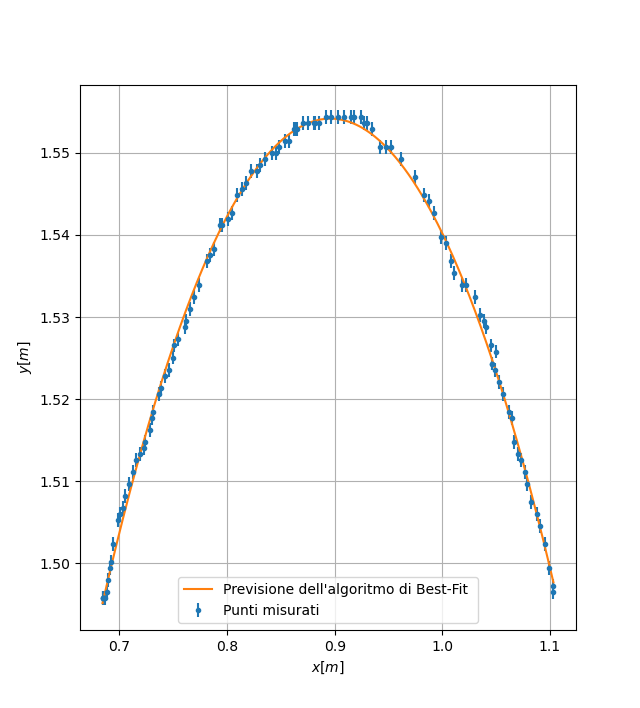
\includegraphics[width=\textwidth]{catenaria_grafico.png}
	\label{plottinobello}
	\caption{Punti misurati e modello di (\ref{cat}) con i parametri dell'algoritmo di best-fit.}
\end{figure}

\begin{figure}
	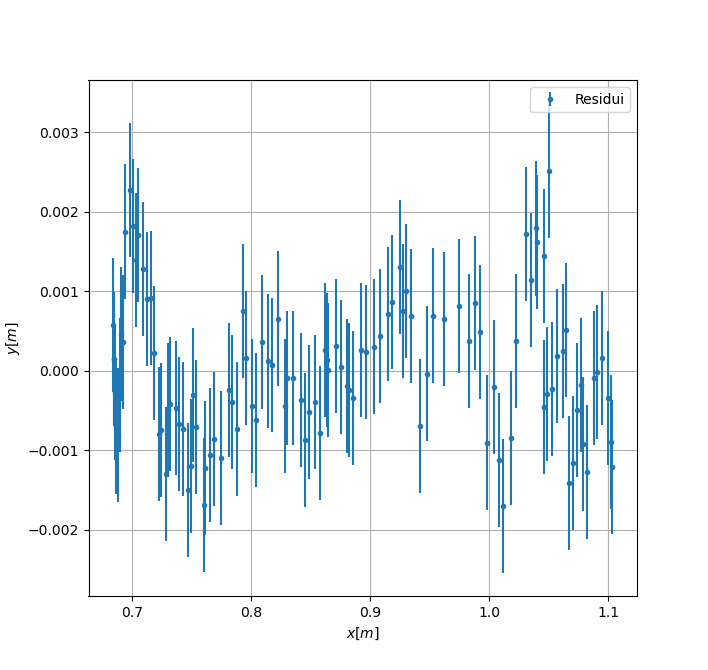
\includegraphics[width=\textwidth]{Catenary_residuals.png}
	\label{residuiumani}
	\caption{Grafico dei residui.}
\end{figure}

\subsection{Algoritmo di Best-Fit}
Per utilizzare l'algoritmo di best fit $"curve\_fit()"$ per l'equazione (\ref{cat}) è stata verificata a posteriori la seguente relazione:
\begin{equation}
\sigma_{y} \gg \left| \frac{dy}{dx} \right| \sigma_{x}
\end{equation}

Nell'intervallo misurato la derivata massima di  (\ref{cat}) con parametri di (Table 1)  delle coordinate campionate è 0.8. 
La relazione (2) è verificata:
\begin{equation}
1.1 [pixel] \gg 0.2[pixel]
\end{equation}


\begin{table}
\centering
	\begin{tabular}{|c|c|c|}

	\hline
		$a$ [m] & $x_0$[m] & $y_0$[m]\\
	\hline
	
		$-0.389\pm0.002$ & $0.8960\pm0.0002$ & $1.943\pm0.002$\\
	\hline
	
	\end{tabular}
	\caption{Valori dei parametri per (\ref{cat}) ottenuti dall'algoritmo di best-fit}
	
\end{table}


\subsection{$X^2$e p-Value}
Il valore dei gradi di libertà è $\nu=108$: abbimo campionato 111 punti e abbiamo utilizzato 3 parametri nel nostro modello. 
Il chi-quadro stimato dall'algoritmo di best-fit è $X^2=120$.
Il p-value corrispondente è $p=0.79$.

\subsection{Errori sistematici}
Dal grafico dei residui (Figure 2) si osserva la presenza di errori sistematici: assunto di avere il modello "corretto" e i parametri "reali", un punto misurato nel grafico dei residui dovrebbe avere il 50\% di trovarsi sopra o sotto lo 0.
Il fatto che ci siano sezioni con 11 punti consecutivi sopra il grafico dovrebbe accadere 1 volta su 2000.  Su un centinaio di punti che questo accada è alquanto improbabile: molto probabilmente è presente un errore sistematico nelle misure. 
Questo potrebbe essere dovuto alla deformazione prospettica, oppure  all'occhio di pesce della lente, oppure a un cattivo capionamento. 

\section{Conclusioni}
Considerato il valore del p-value non ci sono motivi per rigettare il modello dato dall'equazione(\ref{cat}).


\end{document}